\documentclass[thesis.tex]{subfiles}

\section{Problem Statement}
\subsection{Object Detection}
Object detection is a computer vision problem that aims to detect instances of semantic objects of a certain class (such as humans, buildings, cars, etc...) in digital images and videos. Formally, object detection is often defined as: given an input image, produce a correct set of bounding boxes and corresponding labels for each defined object within the image. An example is shown in Figure \ref{fig:obj_example}.

\begin{figure}[htp]
	\centering
	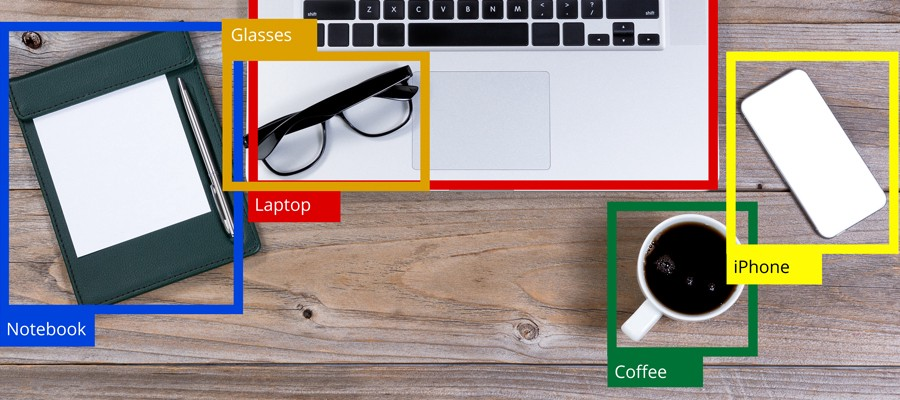
\includegraphics[width=0.7\textwidth]{obj_detection_example.jpeg}
	\caption{An example of object detection}
	\label{fig:obj_example}
\end{figure}

Object detection has a wide range of applications, most notably in surveillance (detecting people, movement,...) and image retrieval (using detected objects as image tags). It is also commonly applied in conjunction with other computer vision tasks, such as classification, eg. an object of a generic class may be detected and then further classified.

The more difficult task of finding the exact bound for objects (as opposed to bounding boxes) is called semantic segmentation.

\subsubsection{Detecting Document Text Regions}
Physical documents, such as books, reports, receipts,... still hold a large amount of information that's often inaccessible to computers. Digitizing these documents can open up a lot of possible applications, such as archiving historic texts, automatically grading exams, or managing personal finance.

\subsection{Large-scale Training of Neural Networks}
